\documentclass[a4paper,12pt]{report}
\addtolength{\oddsidemargin}{-1.cm}
\addtolength{\textwidth}{2cm}
\addtolength{\topmargin}{-2cm}
\addtolength{\textheight}{3.5cm}
\newcommand{\HRule}{\rule{\linewidth}{0.5mm}}
\setcounter{secnumdepth}{5}
\setcounter{tocdepth}{3}
\makeindex

\usepackage{longtable}
\usepackage{graphicx}
\usepackage{makeidx}
\usepackage{hyperref}
\usepackage{verbatim}

\hypersetup{
    colorlinks=true,
    linkcolor=blue,
    filecolor=magenta,      
    urlcolor=cyan,
}


% define the title
\author{Ambitious Design}
\title{ Software Requirements Specifications and Technology Neutral Process Design}
\begin{document}
\setlength{\parskip}{6pt}

% generates the title
\begin{titlepage}

\begin{center}
% Upper part of the page           
\textsc{\LARGE Willburg Outdoor PTY(ltd.)}\\[1.5cm]
\textsc{\Large Smart Image Identifier }\\[1.0cm]
\textsc{\Large Version 1.0 }\\[0.5cm]
% Title
\HRule \\[0.4cm]
{ \huge \bfseries  Software Requirements Specifications and Technology Neutral Process Design}\\[0.4cm]
\HRule \\[0.4cm]
% Author and supervisor
\begin{minipage}{0.4\textwidth}
\begin{flushleft} \large
\emph{Author:}\\
Stephen {Swanepoel}
\end{flushleft}
\end{minipage}
\begin{minipage}{0.4\textwidth}
\begin{flushright} \large
\emph{} \\
u11032091
\end{flushright}
\end{minipage}
\begin{minipage}{0.4\textwidth}
\begin{flushleft} \large
Dian {Veldsman}
\end{flushleft}
\end{minipage}
\begin{minipage}{0.4\textwidth}
\begin{flushright} \large
\emph{} \\
u12081095
\end{flushright}
\end{minipage}
\begin{minipage}{0.4\textwidth}
\begin{flushleft} \large
Killian {Kieck}
\end{flushleft}
\end{minipage}
\begin{minipage}{0.4\textwidth}
\begin{flushright} \large
\emph{} \\
u12252213
\end{flushright}
\end{minipage}


{\large \today}
\end{center}
\end{titlepage}
\footnotesize
\normalsize

\renewcommand{\thesection}{\arabic{section}}
\newpage
\begin{center}
\textsc{\LARGE Software Requirements Specification}\\[1.5cm]
\end{center}



\section{Introduction}
This document aims to set out the functional and non-functional requirements of a system as specified by the Willburg Outdoor PTY(ltd.). The system is required to assess an image by sorting the image into baskets and groupings and then identify if a human is present in the picture. The document will also serve the purpose of communicating the requirements and specifications as needed by the client.

 \subsubsection{Vision}
 The client for this project, Willburg Outdoor PTY(ltd.), has called for the design of an application that will assess an images, identify a human(s) in the image. If a human has been identified by the system, a call must then be set out to warn a user. The main idea behind the project is to be able to alert the user, of the Willburg camera, that a human has been identified so that the user will be informed about the movement around the camera.

\subsubsection{Background}
Rhino poaching is currently at a crisis point. By the end of 2015, the number of African rhinos killed by poachers had increased for the sixth year in a row with at least 1,338 rhinos killed by poachers across Africa in 2015. South Africa has by far the largest population of rhinos in the world and is an incredibly important country for rhino conservation. However rhino poaching levels have dramatically escalated over recent years. \\
\\The South African farm attacks are an ongoing trend of violent attacks on farmers in South Africa. Between 1994 and March 2012, there have been 361,015 murders in South Africa. While the police are supposed to regularly visit commercial farms to ensure security, they claim they cannot provide effective protection due to the wide areas that need to be covered and a lack of funding.\\
\\Willburg Outdoor is company that is passionate about the South Africa. With this passion comes the need to protect its farmers and it animals from those who intend to harm them.The client intends to use the system to fight these two problems by alerting the user of the Willburg camera of the identification in an effort to potentially stop a crime or poaching from accuring. This will hopefully deter future poachers and farm attackers.

\section {Software architecture overview}

	\begin{figure}[htb]
		\centering
		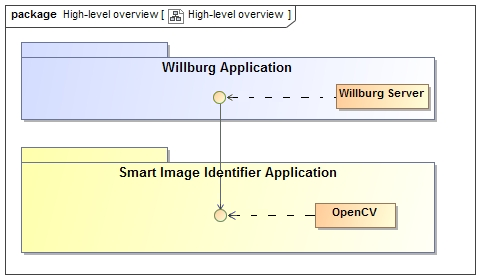
\includegraphics [height= 8cm, width=10cm]{../Diagrams/SystemOverview.png}
		\caption{A high-level overview of the software architecture of the Smart Image Identifier}
	\end{figure}


\section {Overall Software architecture}	
\subsection{Architecture Requirements}
\subsubsection{Access and Integration Requirements}
Any and all interactions by the user will be done through the Willburg Application.
\subsubsection{Quality Requirements}
\paragraph{Performance}
\begin{enumerate}
	\item Images should only be captured and processed if some movement is detected to ensure that the server does not get overloaded.
	\item Images which are processed should not be large in size so they may be processed faster by the server.
	\item The system must be created with the most minimal and efficient coding
	practices possible, given that the result must still be reliable and robust.
\end{enumerate}
\paragraph{Reliability}
\begin{enumerate}
	\item The system must be thoroughly tested on the server side, to
	ensure it will not cause faults or problems. 
	\item The notification warning users will receive must be sent out immediately after the image has been processed in a real-time manner.
\end{enumerate}
\paragraph{Scalability}
\begin{enumerate}
	\item Modular programming should be used in order to ensure that there are no restrictions in terms of the systems ability to be extended and improved upon at later stages.
	\item The server should be able to process multiple images at once to ensure the real-time restriction is met.
\end{enumerate}
\paragraph{Security}
\begin{enumerate}
	\item Depending on the technology being used the various security measures should be in place to ensure the integrity of the server, such as: SQL injections etc.
\end{enumerate}
\paragraph{Flexibility}
\begin{enumerate}
	\item The system should be able to perform correctly even while under strain due to bulk processing without any loss of data.
	\item The system should be modularized to ensure both easy testing of components as well as addition of components without affecting the system.
\end{enumerate}
\paragraph{Maintainability}
\begin{enumerate}
	\item The system should be designed in technologies which offer user support and continuous updates for extra functionality.
	\item The system must be well structured and documented to ensure future developers are able to understand and maintain the system.
	\item The modular design of the system must be such that if changes must be made to a part of the system, only that part itself should be changed.
\end{enumerate}
\paragraph{Auditability}
\begin{enumerate}
	\item All images processed should be logged and traceable(user, date, time etc.) once pushed into the database.
\end{enumerate}
\paragraph{Integrability}
\begin{enumerate}
	\item The system should be designed in a manner which allows for easy 
\end{enumerate}
\paragraph{Cost}
\begin{enumerate}
	\item The tools used to design the system should, as far as possible be open source, free and not require a license.
	\item In certain cases, paid and licensed software may be suitable for specific aspects of the system. 
\end{enumerate}
\paragraph{Usability}
\begin{enumerate}
	\item The Willburg application should be easy for users to interact with regarding the notifications they will be receiving.
\end{enumerate}
\newpage

\subsubsection {Architectural responsibilities}
	
\subsubsection {Architecture Constraints}

\subsection {Architecture design}
This section specifies the very high-level software architecture design, i.e. the software architecture
design for the first level of granularity. It includes the allocation of architectural responsibilities to
architectural components, any tactics which should be used at the current level of granularity to
address quality requirements

\subsubsection {Architectural tactics}
\subsubsection {Architectural components addressing architectural responsibilities}

\subsubsection {Infrastructure}

\section {Application Layer or Framework}
\subsection {Software architecture requirements}
\subsubsection {Quality requirements}
\subsubsection {Architectural responsibilities}

\subsection {Software architecture design for the persistence API}
\subsubsection {Architectural tactics}
\subsubsection {Architectural components}
\subsubsection {Application component concepts and constraints}
\subsubsection {Frameworks and technologies}

\section {Application Server}
The application server is the architectural component within which request for image processing is captured and handled. It is the component hosting the application processes layer of the application.

\subsection {Software architecture requirements}
The architectural requirements include the refined quality requirements and the architectural responsibilities. The architectural constraints for this lower level component are the same as for the system as a whole.

\subsubsection {Quality requirements}
Many of the quality requirements for the system needs to propagated to this lower level component.
In particular, the scalability, maintainability, auditability and deployability requirements specified for the system as a whole are directly applicable for the application server. However some of the higher level requirements needs to be refined for this lower level component.

\paragraph {Flexibility} 
\hfill \break
 Flexibility requirements for the application server include
	\begin{itemize}
		\item The ability to deploy versions of the system with minimum system down-time
		\item The ablity to replace any lower level service with ease
	\end{itemize}
\paragraph {Reliability}
\hfill \break
	Reliability is required around the buisness processes themselves at this level of the business process layer.
	In particular, we require that service contracts are either fully realized as per the service contract or that the calling entity is provided with a reason  for not providing the service.

\paragraph {Security}
\hfill \break
The system does not have potential users accesing methods which should not be accessed and thus does not require authorization. Although, no direct access should given to the database, i.e. data is only accessible through the services offered by the system, with the application server authenticating itself with the database.

\paragraph {Testability}
\hfill \break
All services offered by the system must be testable through automated unit tests, testing components in isolation using mock objects, and automated integration tests where components are integrated within the actual environment.
These functional tests should verify that the service is provided if all pre-conditions are met and that all post-conditions hold true once the service has been provided.

\paragraph {Flexibility}
\hfill \break
All services offered by the system must be testable through automated unit tests, testing components in isolation using mock objects, and automated integration tests where components are integrated within the actual environment.
These functional tests should verify that the service is provided if all pre-conditions are met and that all post-conditions hold true once the service has been provided.

\subsubsection {Architectural responsiblities}

	\begin{figure}[htb]
		\centering
		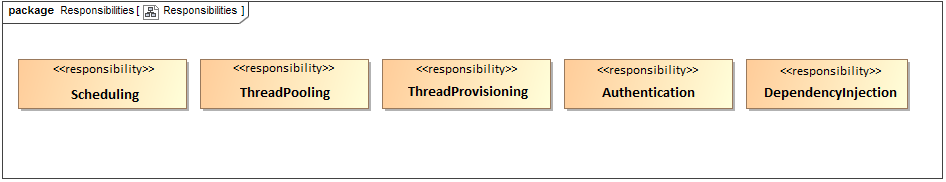
\includegraphics  [scale=0.5]{../Diagrams/applicationServerResponsibiltiesZ.png}
		\caption{The architectural responsibilities of the application server}
	\end{figure}


\subsection {Architecture design}
\subsubsection {Tactics}
\paragraph {Flexibility tactics}
\hfill \break
The chosen application server should concretely address the flexibility requirements. The application server should support 
	\begin {itemize}
		\item hot-deployment, i.e. the ablility to deploy new versions of the system into the live enviroment with minimum downtime
		\item component (contract) based software development with dependency injection.
	\end {itemize}
 
\paragraph {Maintainability tactics}
\hfill \break
The application server should be based on a public standard with multiple implementations including at least one open-source implementation of the standard.
being available.

\paragraph {Reliability tactics}
\hfill \break
The application server must provide support for transactions which may enlist a variety of resources. In particular, the system requires the ability to commit and rollback across the persistence provider (i.e. the database).The transaction support should be declarative, i.e. that one specifies the transactional requirements and does not hard code transaction boundaries. This has the advantage that services can be reused across different business processes requiring different transactional boundaries. 

\paragraph {Security}
\hfill \break

\paragraph {Auditability tactics}
\hfill \break
Auditability is an important quality requirement and needs to be addressed in the business processes layer. The auditability specification must be maintainable. To this end, the application server must support specifying logging logic (advices) as cross-cutting concerns within aspects or at least provide the ability to apply logging via interception.

\paragraph {Testability tactics }
In order to be able to reuse unit tests as integration and regression tests the frameworks and technologies used at the business process layer must support dependency injection. The application server must support hosting code which can be tested outside the application server

\subsubsection {Architectural components}
	\begin{figure}[htb]
		\centering
		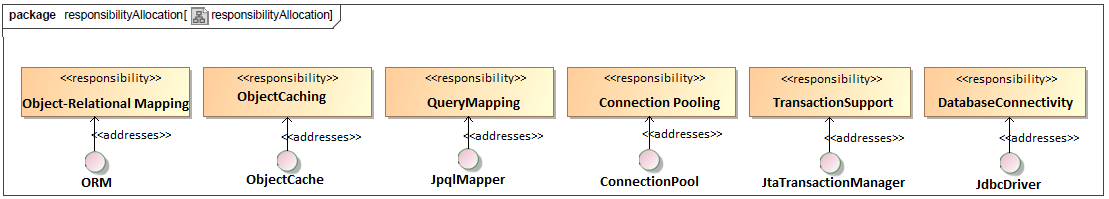
\includegraphics [scale=0.5]{../Diagrams/PersistanceResponsibiltiesAllocationZ.png}
		\caption{The abstract components to which the architectural responsibilities are assigned}
	\end{figure}

\subsubsection {Application Component Concepts and Constraints}
The central concept which will be used to specify application logic (the business processes) are the
concepts of
	\begin {itemize}
		\item a \textit{service contract} which encodes the requirements for a service
		\item a \textit{service} which encodes the concrete implementation of a service. 
	\end {itemize}
These services which encapsulate the processes will be constrained to be stateless, i.e. no state
is maintained across service requests.
Long living state is maintained in domain objects which are typically persisted and which should
not have any business logic.



\subsubsection {Frameworks and technologies}
JBoss
Netty or MINA


\paragraph {Concrete realization of architectural components}
\hfill \break
The Java-EE reference architecture addresses largely all the architectural responsibilities assigned to the application server.

\paragraph {Tactics}
\hfill \break
With the exception of full aspect-oriented programming, Java-EE-7 supports all architectural tactics specified in the software architecture design for the application server.

\subparagraph {Concrete realization of flexibility tactics  within Java-EE}
\hfill \break
Java-EE supports
	\begin {itemize}
		\item Java-EE is a component-based framework requiring decoupling through interfaces/contracts.
		\item Hot-deployment is supported by most application servers including the most widely used
open-source application servers like JBoss and Glassfish.
		\item CDI (Context and Dependency Injection) is fully supported within Java-EE with dependency
injection requested via @Inject annotations.
	\end {itemize}

\subparagraph {Concrete realization of maintainability tactics  within Java-EE}
Java-EE is based on a public standard which is widely supported and hence the support for this technology is secured for the foreseeable future. The technology puts a rigorous framework in place for defining services within stateless session beans which are decoupled through interfaces/contracts. Maintainability is enhanced by dependency injection which allows for changing service providers at any level of granularity without making code changes. Furthermore the replacement of such new
or improved functionality can be done within a live system using hot deployment.

\subparagraph {Concrete realization of reliability tactics  within Java-EE}
\hfill \break
Java-EE uses thread-pooling, object-pooling, connection-pooling and clustering to improve scalability.

\subparagraph {Concrete realization of security tactics  within Java-EE}
\hfill \break

\subparagraph {Concrete realization of testability tactics  within Java-EE}
\hfill \break

\paragraph {Application component concepts and constraints}


\section {Persistence API}
The persistence API provides abstracted access to a persistence to a persistence provider (database)
whilst remaining decoupled from the database technology as well as the concrete database selected
for the system. It also implements a range of tactics in order to concretely address quality requirements required from the persistence domain.

\subsection {Software architecture requirements}
The architectural requirements for the persistence API include the refined quality requirements and
the architectural responsibilities. The architectural constraints for this lower level component are
the same as for the system as a whole.

\subsubsection {Quality requirements}
Particularly, scalability, reliability, flexibility and maintainability are important for the persistence API.

\paragraph {Scalability}
\hfill \break
Chosen persistance API should allow the future scaling of the infrastructure.

\paragraph {Reliability}

\paragraph {Flexibility}
\hfill \break
The chosen persistance API should be able to adapt to the rapidly changing persistance domain. This is especially important when it comes to different methods, such as relational and non-relational(NoSQL) databases, of storing data. \newline 
The chosen persistance API should provide a layer of abstraction, allowing any transaction manager to be used. It is also important that the chosen persisitance API should not be locked into any specific persistance technology.

\paragraph {Maintainability}
\hfill \break
The chosen persistance API should be a widely used API, it should also be in an advanced stage in its development life cycle. This is in order to ensure that information about the API is readily availble and widely understood. Inorder to be able to easily switch from one API implementation to another and to be able to gaurd against abondoning of technologies, if it is required for long term maintance, the API chosen should be a an open standard.

\paragraph {Performance}

\subsubsection {Architectural responsibilities}
	\begin{figure}[htb]
		\centering
		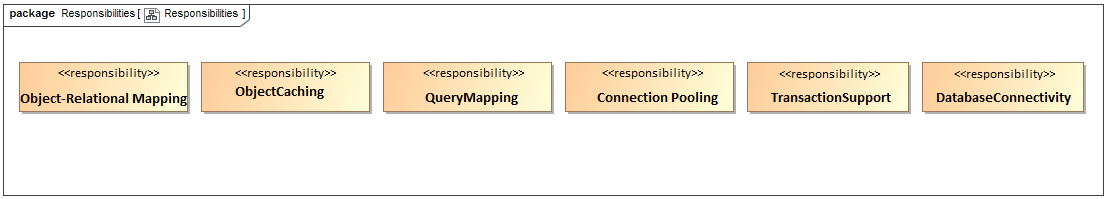
\includegraphics  [scale=0.5]{../Diagrams/PersistanceResponsibiltiesZ.png}
		\caption{The architectural responsibilities of the persistence API}
	\end{figure}

\subsection {Software architecture design for the persistence API}
\subsubsection {Architectural tactics}
The persistence API should use
	\begin {itemize}
		\item \textit{Object-Relational Mapping} to reduce code bulk, improve maintainability and allow for decoupling from the 		persistence provider
		
		\item \textit{Query mapping} from queries across a graph of Java objects onto the database queries used in the selected database technology and provider

		\item \textit{Object caching} to improve scalability and performance

		\item \textit{Transactions} with 2-phase commit to improve reliability of processes.

		\item \textit{Connection pooling} to improve performance and scalability.
	\end {itemize}

\subsubsection {Architectural components}

\subsubsection {Application component concepts and constraints}
	\begin {itemize}
		\item \textit{Domain objects} (entities) which host long-living state. These entities hold no logic and is known as Plain Old Java Objects (POJO's) in the Java architecture.

		\item \textit{Queries across object graph of domain objects } through which the required information of state in the domain objects retreived or modified.
	\end {itemize}
\subsubsection {Frameworks and technologies}
A JPA (Java Persistence API) provider will be used as a persistence API. The concrete implementation used for the chosen API is Hibernate. Hibernate has support for both relational and non-relational databases. IT is also widely used, has good community support and is well documented. Performance plays a significant role in the system as it is a real-time system and Hibernate is one of the top open-source persistance implementations in terms of performance. \newline
Because JPA is a widely used and supported standard it has many implementations, such as:
	\begin {itemize} 
		\item iBATIS
		\item Hibernate
		\item EclipseLink
	\end {itemize} 

The persistence context (EntityManager) will be dependency injected into services requiring access to persistent data. JPA provider do implement

	\begin {itemize} 
		\item \textit{Object-relational mapping} including mapping of relationships between objects via a provided ORM
		\item \textit{query mapping} from object-oriented queries across the domain objects graph to queries for a specific database provider (e.g. ontio SQL)
		\item\textit{object caching} (within the persistence context)
		\item \textit{transaction support} though the Java Transation API
		\item \textit{connection pooling} through a JCA connector based implementation of a JDBC driver
	\end {itemize} 

Queries will be specified as Spring Data JPA queries.

\end{document}